

\tikzset{every picture/.style={line width=0.75pt}} %set default line width to 0.75pt        

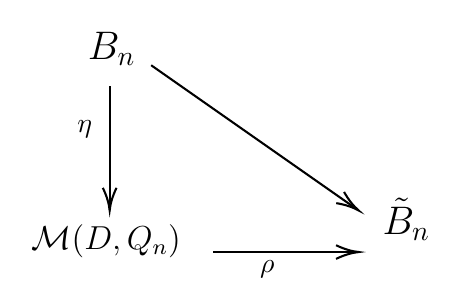
\begin{tikzpicture}[x=0.75pt,y=0.75pt,yscale=-1,xscale=1]
%uncomment if require: \path (0,877); %set diagram left start at 0, and has height of 877

%Straight Lines [id:da3495190020906457] 
\draw    (190,130) -- (190,188) ;
\draw [shift={(190,190)}, rotate = 270] [color={rgb, 255:red, 0; green, 0; blue, 0 }  ][line width=0.75]    (10.93,-3.29) .. controls (6.95,-1.4) and (3.31,-0.3) .. (0,0) .. controls (3.31,0.3) and (6.95,1.4) .. (10.93,3.29)   ;
%Straight Lines [id:da11668079361738581] 
\draw    (210,120) -- (308.36,188.85) ;
\draw [shift={(310,190)}, rotate = 214.99] [color={rgb, 255:red, 0; green, 0; blue, 0 }  ][line width=0.75]    (10.93,-3.29) .. controls (6.95,-1.4) and (3.31,-0.3) .. (0,0) .. controls (3.31,0.3) and (6.95,1.4) .. (10.93,3.29)   ;
%Straight Lines [id:da13478561325303762] 
\draw    (240,210) -- (308,210) ;
\draw [shift={(310,210)}, rotate = 180] [color={rgb, 255:red, 0; green, 0; blue, 0 }  ][line width=0.75]    (10.93,-3.29) .. controls (6.95,-1.4) and (3.31,-0.3) .. (0,0) .. controls (3.31,0.3) and (6.95,1.4) .. (10.93,3.29)   ;

% Text Node
\draw (178,102.4) node [anchor=north west][inner sep=0.75pt]  [font=\Large]  {$B_{n}$};
% Text Node
\draw (151,195.4) node [anchor=north west][inner sep=0.75pt]  [font=\large]  {$\mathcal{M}( D,Q_{n})$};
% Text Node
\draw (320,182.4) node [anchor=north west][inner sep=0.75pt]  [font=\Large]  {$\tilde{B}_{n}$};
% Text Node
\draw (261,212.4) node [anchor=north west][inner sep=0.75pt]    {$\rho $};
% Text Node
\draw (173,145.4) node [anchor=north west][inner sep=0.75pt]    {$\eta $};


\end{tikzpicture}